\mode*
\begin{frame}
 	\section{Experimental Results}
 	\frametitle{Experimental Results}
	\textbf{Approaches and Settings}
	\begin{itemize}
		\item k-Nearest Neighbors
		\item Na\"ive Bayes
		\item Decision Tree
		\item Neural Network
		\item Ensemble
	\end{itemize}
\end{frame}

\begin{frame}
	\frametitle{k-Nearest Neighbors}
	\begin{itemize}
		\item parameter search on a leave-one-out cross validation
		\item k=30 best (accuracy)
		\item distance measure = euclidean distance
		\item no distance weighting => better results
	\end{itemize}
\end{frame}

\begin{frame}
	\frametitle{Na\"ive Bayes}
	Another approach is the Na\"ive Bayes classifier. Despite some
	attributes obviously not being independent, it was still employed
	because it proved to be useful in other areas as well.
\end{frame}

\begin{frame}[fragile]
	\frametitle{Decision Tree}
	\begin{itemize}
		\item prunes J48-decision tree
		\item confidence factor =  \(c=0.045\)
		\item found by utilizing WEKAs capabilities of linear
		parameter search
	\end{itemize}
\end{frame}

\begin{frame}[fragile]
	\frametitle{Neural Network}
	\begin{itemize}
		\item multilayer perceptron
		\item 13 input neurons (features)
		\item hidden layer of 17 neurons
		\item output layer with three neurons (classes)
		\item learning rate: \(\alpha=0.1\)
		\item momentum:  \(m=0.1\) (backpropagation algorithm)
		\item linear search for parameters: hidden neurons, learning rate and momentum
	\end{itemize}
\end{frame}

\begin{frame}
	\frametitle{Ensemble}
	In hope for enhanced results by combining the strenghts of the
	different classifiers, all models were combined into an ensemble. The
	vote of the whole ensemble was found by conducting a majority voting.
\end{frame}


\begin{frame}
	\frametitle{Results}
	\begin{itemize}
		\item 10-fold cross validation
	\end{itemize}
	\begin{figure}[h]
		\centering
		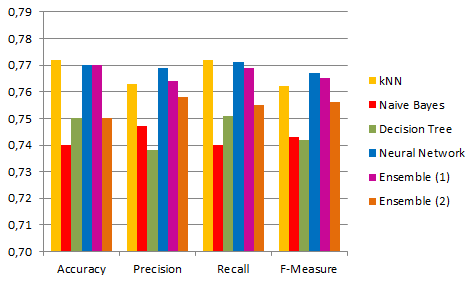
\includegraphics[width=0.8\columnwidth]{../../charts/results.png}
		\caption{Evaluation metrics of the different classifiers}
		\label{fig:result}
	\end{figure}
\end{frame}

\begin{frame}
	\begin{table}[h]
		\centering
		\caption{Confusion matrix of the ensemble}
		\label{tab:mat-vote}
		\resizebox{\columnwidth}{!}{
			\begin{tabular}[c]{c|ccc||c}
				classified \(\rightarrow\) & \textbf{Low} & \textbf{Medium} & \textbf{High} & Total\\ \hline
				Low & \textcolor{blue}{1125} & 126 & 8 & 1259 \\
				Medium & 160 & \textcolor{blue}{305} & 57 & 522 \\
				High & 15 & 95 & \textcolor{blue}{103} & 213 \\ \hline \hline
				Total & 1300 & 526 & 168 & 1994 \\
			\end{tabular}
		}
	\end{table}
\end{frame}


\begin{frame}
	\frametitle{Recall}	
	\begin{figure}[h]
		\centering
		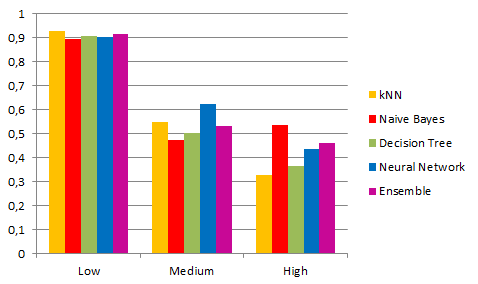
\includegraphics[width=0.8\columnwidth]{../../charts/recall.png}
		\caption{Recall of the different classifiers}
		\label{fig:recall}
	\end{figure}
\end{frame}


\subsection{Discussion and Outlook}

As shown in figures \ref{fig:result} and \ref{fig:recall}, each of the
classifiers does indeed have its own strengths and weaknesses.
While k-Nearest Neighbors excels in terms of accuracy and overall
recall, the Neural Network performs best in terms of precision and
f-measure. A fairly interesting observation can be made when looking
at the different recall values with respect to the class "High":
Here, the Na\"ive Bayesian classifier achieves by far the most impressive
results when compared to the other models. This turns out to be a
contrast to the overall scores of this classifier, which are merely average.

Contrary to our initial believe, that the combination of all
classifiers into an ensemble would enhance the results, we have to
admit, that this was not quite the case. Overall, the ensemble always
ranks among the best, but it never reached top spot in any
category. In fact it turned out to be worse than the Neural Network in
every category except for the recall with respect to the class "High".

This seemingly paradox incidence can be explained when
thinking about the effects of combining different classifiers: When
merging the different models, not only the strengths are combined but
also the weaknesses. This results in the observed pattern: By
combining the classifiers, the strengths and weaknesses average out,
thus the obtained results are also average.

It should be noted however, that there are methods to bias the results
of the ensemble more towards the stronger side of the spectrum.
By giving each of the voters a different weight, one could emphasize the
strengths of one classifier and mitigate the weaknesses of
another.

\noindent Nevertheless, developing such a method to intelligently balance the weights of an
ensemble would most likely require further study, which
could form the basis of another research project.

\mode<all>